% --------------------------------------------------------------
% This is all preamble stuff that you don't have to worry about.
% Head down to where it says "Start here"
% --------------------------------------------------------------
 
\documentclass[12pt]{article}
\usepackage{makecell}
\usepackage[export]{adjustbox}
 
\usepackage[margin=1in]{geometry} 
\usepackage{amsmath,amsthm,amssymb}
\usepackage[margin=1in]{geometry} 
\usepackage{amsmath,amsthm,amssymb}
\usepackage{float}
\usepackage[T1]{fontenc} %escribe lo del teclado
\usepackage[utf8]{inputenc} %Reconoce algunos símbolos
\usepackage{lmodern} %optimiza algunas fuentes
\usepackage{graphicx}
\graphicspath{ {images/} }
\usepackage{hyperref} % Uso de links
 \usepackage{ragged2e}
\newcommand{\N}{\mathbb{N}}
\newcommand{\Z}{\mathbb{Z}}
 
\newenvironment{theorem}[2][Theorem]{\begin{trivlist}
\item[\hskip \labelsep {\bfseries #1}\hskip \labelsep {\bfseries #2.}]}{\end{trivlist}}
\newenvironment{lemma}[2][Lemma]{\begin{trivlist}
\item[\hskip \labelsep {\bfseries #1}\hskip \labelsep {\bfseries #2.}]}{\end{trivlist}}
\newenvironment{exercise}[2][Exercise]{\begin{trivlist}
\item[\hskip \labelsep {\bfseries #1}\hskip \labelsep {\bfseries #2.}]}{\end{trivlist}}
\newenvironment{problem}[2][Problem]{\begin{trivlist}
\item[\hskip \labelsep {\bfseries #1}\hskip \labelsep {\bfseries #2.}]}{\end{trivlist}}
\newenvironment{question}[2][Question]{\begin{trivlist}
\item[\hskip \labelsep {\bfseries #1}\hskip \labelsep {\bfseries #2.}]}{\end{trivlist}}
\newenvironment{corollary}[2][Corollary]{\begin{trivlist}
\item[\hskip \labelsep {\bfseries #1}\hskip \labelsep {\bfseries #2.}]}{\end{trivlist}}

\newenvironment{solution}{\begin{proof}[Solution]}{\end{proof}}
 
\begin{document}
 
% --------------------------------------------------------------
%                         Start here
% --------------------------------------------------------------
 
\title{CSE-4111, Artificial Intelligent Lab}
\author{Mirajul Mohin, Roll: FH-28\\ %replace with your name
}

\maketitle
\section*{\centering Online Roommate Allocation Problem}
\centering\textbf{Guangda Huzhang\textsuperscript1, Xin Huang\textsuperscript2, Shengyu Zhang\textsuperscript3, Xiaohui Bei\textsuperscript4}\\
\textsuperscript{1,4}School of Physical and Mathematical Sciences, Nanyang Technological University\\
\textsuperscript{2,3}Department of Computer Science and Engineering, The Chinese University of Hong Kong \\
\raggedright
\section*{Problem Definition}
\justify This research introduces an online algorithm for roommate market model. Let, a roommate market model contains n fixed rooms and 2n number of agents. Now the problem is to assign a room for each person upon his/her arrival and thus after termination each room contains exactly two persons. Two things need to be satisfied (1) maximizing social welfare (2) satisfying stability property. It first addresses an online algorithm (where each room contains exactly two person) which works in polynomial time having a constant competitive ratio. And then extends this for the case where each room can contain c > 2 people.
\section*{Method}
Here, given a set of n rooms $R = \{r\textsubscript1, r\textsubscript2, r\textsubscript3,....,r\textsubscript n\}$, a set of 2n agents $I = \{1,2,3,....2n\}$, a happiness matrix $H = \{h\textsubscript{ij} | i, j \epsilon I, i \ne j\}$, a valuation matrix $V = \{v\textsubscript{ir} | i \epsilon I , r \epsilon R\}$ and the outcome of this model is $A = \{(i,j,r)\}$, which means that agent $i$ is assigned to agent $j$ in room $r$.
Social welfare of an allocation $A$ is $SW(A) = \sum \textsubscript{$(i,j,r) \epsilon A$} (h\textsubscript{ij} + h\textsubscript{ji} + v\textsubscript{ir} + v\textsubscript{jr})$\\\\
Here it is assumed an online setting where each agent arrive in a uniform random order and immediately after arrival agents need to be assigned to a room.\\\\
For the first part, total number of agents is $2n$ where total number of rooms is $n$. So, each room will contain exactly two people. For the second part, total number of agents is $cn$, where $n$ is the total room number. So, each room can contain $c$ number of people.\\\\
The main goal is to find an allocation that maximizes social welfare $SW(A)$, where the expectation is taken over both the randomness of the algorithm and the random arriving order of the agents.
\newpage
\section*{Input/Output (Part-1)}
\begin{figure}[H]
	\begin{minipage}{.5\linewidth}
		\centering
		\[V=\left[\begin{array}{cc}
		5 & 2 \\
		7 & 9 \\
		2 & 1 \\
		7 & 9
		\end{array}\right]\]
		Valuation matrix $V$
	\end{minipage}%
	\begin{minipage}{.5\linewidth}
		\centering
		\[H=\left[\begin{array}{cccc}
		0 & 5 & 3 & 7 \\
		2 & 0 & 5 & 3 \\
		5 & 3 & 0 & 1 \\
		7 & 3 & 2 & 0
		\end{array}\right]\]
		Happiness matrix $H$
	\end{minipage}
\end{figure}
\noindent
For n = 2, total number of rooms is 2, total number of agents is 4. So the dimension of Valuation matrix is 4 x 2 (2n x n) and the dimension of Happiness matrix is 4 x 4 (2n x 2n).\\\\
\noindent If four agents come following 0, 1, 3, 2 this sequence, for two matrix mentioned above my implementation gives two allocation ([0, 3], 0) and ([1, 2], 1). That means agent-0, agent-3 will be in room-0 and agent-1, agent-2 will be in room-1. 
\begin{figure}[H]
	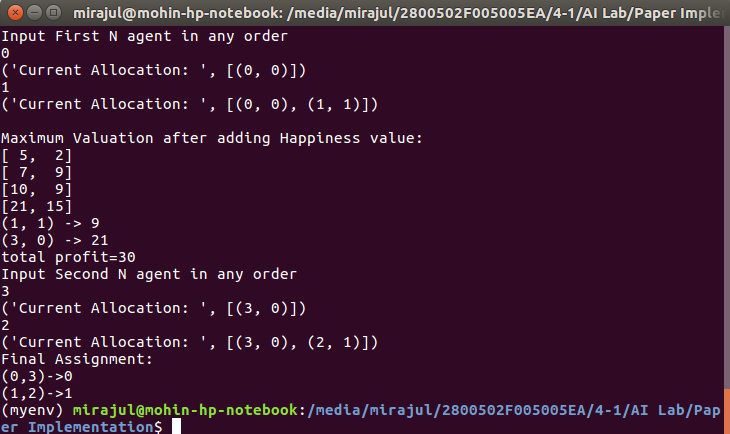
\includegraphics[width=\textwidth, center]{1}
	\caption{Figure showing allocation for above input}
	\label{fig:figure2}
\end{figure}

\noindent
The above figure shows an allocation for 4 agents, 2 rooms and for the above Valuation and Happiness matrix. 
\newpage
\section*{Input/Output (Part-2)}
This part generalizes the previous online market problem where each room can take c people, where c > 2. Here, total number of agent is $cn$, number of rooms is $n$. So, each room will contain $c$ number of people. It just uses the previous algorithm to run $c$ times for updated $V$ matrix.
\begin{figure}[H]
	\begin{minipage}{.5\linewidth}
		\centering
		\[V=\left[\begin{array}{cc}
		5 & 2 \\
		7 & 9 \\
		2 & 1 \\
		7 & 9 \\
		6 & 2 \\
		5 & 3 \\
		\end{array}\right]\]
		Valuation matrix $V$
	\end{minipage}%
	\begin{minipage}{.5\linewidth}
		\centering
		\[H=\left[\begin{array}{cccccc}
		0 & 5 & 3 & 7 & 2 & 9\\
		2 & 0 & 5 & 3 & 6 & 1\\
		5 & 3 & 0 & 1 & 4 & 8\\
		7 & 3 & 2 & 0 & 3 & 5\\
		2 & 5 & 3 & 9 & 0 & 7\\
		3 & 2 & 1 & 5 & 9 & 0
		\end{array}\right]\]
		Happiness matrix $H$
	\end{minipage}
\end{figure}
\noindent
For n = 2 and c = 3 , total number of rooms is 2, total number of agents is 6. So the dimension of Valuation matrix is 6 x 2 (cn x n) and the dimension of Happiness matrix is 6 x 6 (cn x cn).\\\\
\noindent If six agents come following 0, 1, 3, 2, 5, 4 this sequence, for two matrix mentioned above my implementation gives two allocation ([0, 3, 4], 0) and ([1, 2, 5], 1). That means agent-0, agent-3 and agent-4 will be in room-0 and agent-1, agent-1, agent-2 and agent-5 will be in room-1. 
\begin{figure}[H]
	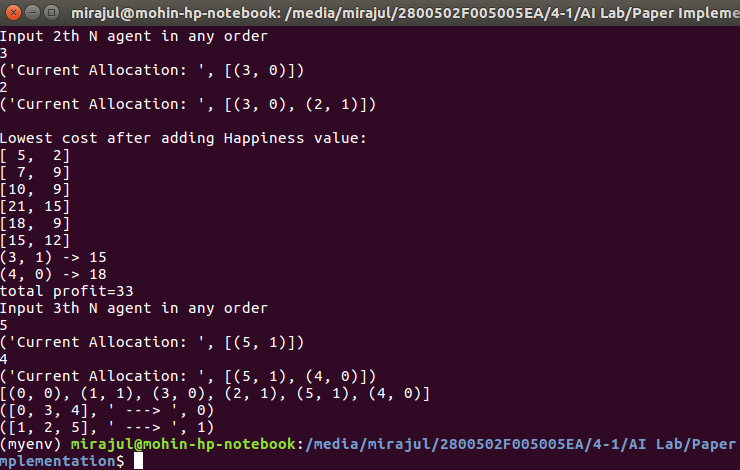
\includegraphics[width=0.95\textwidth, center]{2}
	\caption{Figure showing allocation for above input}
	\label{fig:figure2}
\end{figure}


\newpage

\section*{Discussion}
Three algorithms, ONLINEMATCHING(n, R),  ONLINEROOMMATE (n, H, V) and ONLINECBEDROOMMATE (n, H, V) are used. Here ONLINEMATCHING(n, R) is a polynomial time algorithm having $c\textsubscript b$ the competitive ratio, where $c\textsubscript b = \frac{\ln 5 - 0.8}{5} \approx 0.1618$ \textit{[Kesselheim et al., 2013]}\\\\
They have proposed ONLINEROOMMATE (n, H, V) which is a polynomial time constant $\frac{c\textsubscript b}{4}$-competitive algorithm [$c\textsubscript b = \frac{\ln 5 - 0.8}{5} \approx 0.1618$]. Constant competitive ratio has been calculated comparing with the same off-line allocation. \\\\
The last one, ONLINECBEDROOMMATE (n, H, V), is the extended version of proposed ONLINEROOMMATE (n, H, V) algorithm. This algorithm has competitive ratio $\frac{c\textsubscript b (c - 1)}{c\textsuperscript 3}$ [$c\textsubscript b = \frac{\ln 5 - 0.8}{5} \approx 0.1618$].\\\\
The next part of this research addresses another algorithm where rooms are with different capacities. Besides, they have proved some stability conditions and some other things related to it. 
% --------------------------------------------------------------
%     You don't have to mess with anything below this line.
% --------------------------------------------------------------
 
\end{document}